\subsection{The Area of a Triangle}

Given a triangle $T$ with corners $(x_i, y_i, z_i)$, $(x_j, y_j, z_j)$, and $(x_k, y_k, z_k)$, the area of the triangle $A_T$ is
\[
    A_T = \frac{1}{2} \left| \begin{pmatrix}
        x_j - x_i \\ y_j - y_i \\ z_j - z_i
    \end{pmatrix} \times \begin{pmatrix}
        x_k - x_i \\ y_k - y_i \\ z_k - z_i
    \end{pmatrix} \right| = \frac{1}{2} \begin{vmatrix}
        (y_j - y_i)(z_k - z_i) - (y_k - y_i)(z_j - z_i) \\
        (x_k - x_i)(z_j - z_i) - (x_j - x_i)(z_k - z_i) \\
        (x_j - x_i)(y_k - y_i) - (x_k - x_i)(y_j - y_i)
    \end{vmatrix}.
\]

In the 2D case where $z_i = z_j = z_k$, this becomes\footnote{Technically, this could be the negative of the area and to get the actual area you need to take an absolute value. Solving it this way makes the next steps easier, however.}
\[
    A_T = \frac{1}{2} \left[(x_j - x_i)(y_k - y_i) - (x_k - x_i)(y_j - y_i)\right] = \frac{1}{2} \left(x_i y_j + x_j y_k + x_k y_i - x_i y_k - x_k y_j - x_j y_i\right).
\]

\subsection{The Damping Matrix}

The damping matrix $\mathbf{D}$ is defined so that
\[
    d_{i, j} = \int_\Omega \psi_i \psi_j dA.
\]
I consider a triangle $T$ with both $v_i$ and $v_j$ as vertices to $T$. From the solution for $T$, we know
\[
    d_{i, j} = \sum_{\{T: v_i, v_j \in T\}} \int_T \psi_i \psi_j dA.
\]

\begin{figure}[t!]
    \centering
    \caption{Transformation from $T^0$ to $T$.}

    \begin{subfigure}{0.27\textwidth}
        \resizebox{\textwidth}{!}{%
        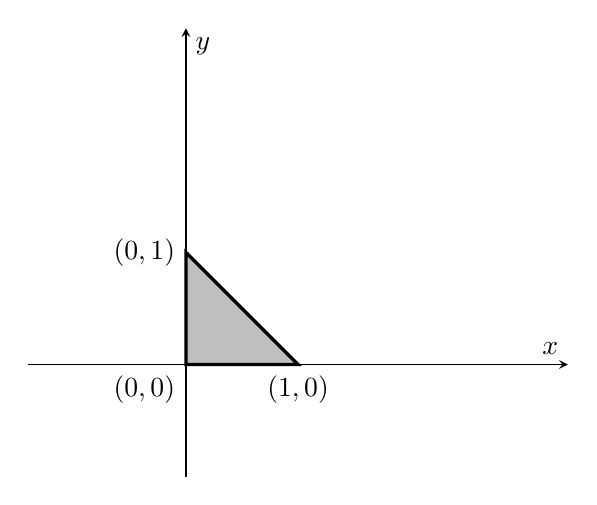
\begin{tikzpicture}
            \begin{axis}[xlabel=$x$, ylabel=$y$, axis lines=middle, xtick={6}, ytick={6}, no marks, axis equal, xmin=-1, xmax=3, ymin=-1, ymax=3]
                \draw[very thick, fill=lightgray] (0,0) node[anchor=north east]{$(0, 0)$}
                -- (1,0) node[anchor=north]{$(1, 0)$}
                -- (0,1) node[anchor=east]{$(0, 1)$}
                -- cycle;
            \end{axis}
        \end{tikzpicture}%
        }
        \caption{Initial triangle $T^0$}%
    \end{subfigure} \quad
    \begin{subfigure}{0.27\textwidth}%
        \resizebox{\textwidth}{!}{%
        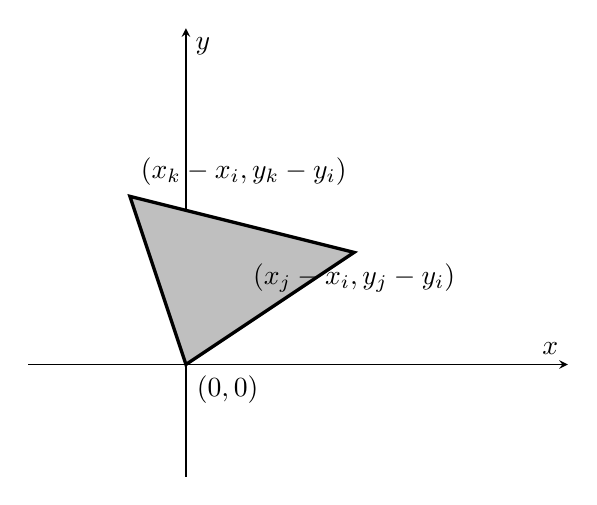
\begin{tikzpicture}
            \begin{axis}[xlabel=$x$, ylabel=$y$, axis lines=middle, xtick={6}, ytick={6}, no marks, axis equal, xmin=-1, xmax=3, ymin=-1, ymax=3]
                \draw[very thick, fill=lightgray] (0,0) node[anchor=north west]{$(0, 0)$}
                -- (1.5,1) node[anchor=north]{$(x_j - x_i, y_j - y_i)$}
                -- (-0.5,1.5) node[anchor=south west]{$(x_k - x_i, y_k - y_i)$}
                -- cycle;
            \end{axis}
        \end{tikzpicture}%
        }
        \caption{Rotated and scaled}%
    \end{subfigure} \quad
    \begin{subfigure}{0.27\textwidth}%
        \resizebox{\textwidth}{!}{%
        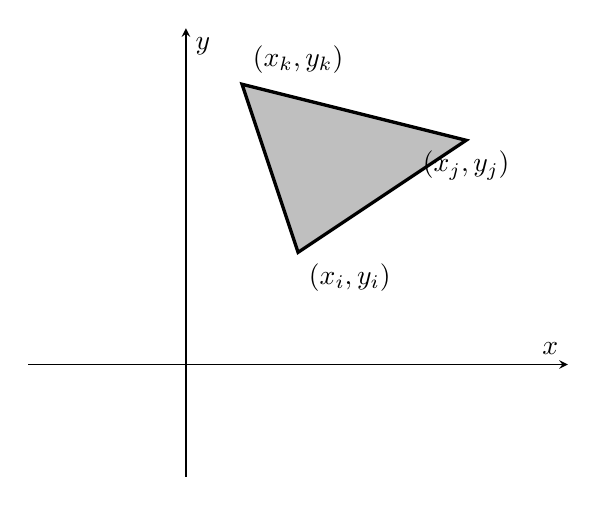
\begin{tikzpicture}
            \begin{axis}[xlabel=$x$, ylabel=$y$, axis lines=middle, xtick={6}, ytick={6}, no marks, axis equal, xmin=-1, xmax=3, ymin=-1, ymax=3]
                \draw[very thick, fill=lightgray] (1,1) node[anchor=north west]{$(x_i, y_i)$}
                -- (2.5,2) node[anchor=north]{$(x_j, y_j)$}
                -- (0.5,2.5) node[anchor=south west]{$(x_k, y_k)$}
                -- cycle;
            \end{axis}
        \end{tikzpicture}%
        }
        \caption{Translated to $T$}
    \end{subfigure}

    \label{fig:T0-to-T}
\end{figure}

To calculate this integral over $T$, we will first define an affine transformation from $T^0$ to $T$ where $T^0$ is a right triangle with $v_i = (0, 0)$, $v_j = (1, 0)$, and $v_k = (0, 1)$ (Figure \ref{fig:T0-to-T}). To map from $\tilde{x}, \tilde{y}$ on $T^0$ to $T$, we first scale and rotate according to the linear transformation
\[
    \begin{pmatrix}
        x_j - x_i & x_k - x_i \\
        y_j - y_i & y_k - y_i \\
    \end{pmatrix} \begin{pmatrix}
        \tilde{x} \\ \tilde{y}
    \end{pmatrix}
\]
then add $(x_i, y_i)^\top$ to get to $T$. Therefore, to get from $\tilde{x}, \tilde{y}$ on $T^0$ to $x, y$ on $T$, we use
\begin{align*}
    x = x_i + (x_j - x_i) \tilde{x} + (x_k - x_i) \tilde{y} \\
    y = y_i + (y_j - y_i) \tilde{x} + (y_k - y_i) \tilde{y}.
\end{align*}
The Jacobian of this transformation
\[
    \begin{pmatrix}
        x_j - x_i & x_k - x_i \\
        y_j - y_i & y_k - y_i
    \end{pmatrix}
\]
has determinant
\[
    \begin{vmatrix}
        x_j - x_i & x_k - x_i \\
        y_j - y_i & y_k - y_i
    \end{vmatrix} = (x_j - x_i)(y_k - y_i) - (x_k - x_i)(y_j - y_i) = 2 A_T.
\]
Therefore, we get
\[
    \int_T \psi_i(x, y) \psi_j(x, y) dydx = 2 A_t \int_{T^0} \psi_i(\tilde{x}, \tilde{y}) \psi_j(\tilde{x}, \tilde{y}) d\tilde{y}d\tilde{x}x.
\]

On $T^0$, we have
\[
    \psi_i (\tilde{x}, \tilde{y}) = 1 - \tilde{x} - \tilde{y} \quad \text{and} \quad \psi_j (\tilde{x}, \tilde{y}) = \tilde{x}.
\]
Therefore, we know
\begin{align*}
    \int_T \psi_i(x, y) \psi_i(x, y) dydx &= 2 A_T \int_{T^0} \psi_i(\tilde{x}, \tilde{y}) \psi_i(\tilde{x}, \tilde{y}) d\tilde{y}d\tilde{x} \\
    &= 2 A_T \int_0^1 \int_0^{1 - \tilde{x}} (1 - \tilde{x} - \tilde{y})^2 d\tilde{y}d\tilde{x} \\
    &= 2 A_T \int_0^1 \int_0^{1 - \tilde{x}} \left[ 1 - 2 \tilde{x} - 2 \tilde{y} + 2 \tilde{x} \tilde{y} + \tilde{x}^2 + \tilde{y}^2 \right] d\tilde{y}d\tilde{x} \\
    &= \frac{2}{3} A_T \int_0^1 (1 - \tilde{x})^3 d\tilde{x} \\
    &= \frac{2}{3} A_T \int_1^0 \hat{x}^3 (-1) d\hat{x}, \quad \hat{x} = 1 - \tilde{x} \\
    &= \frac{1}{6} A_T
\end{align*}
and
\begin{align*}
    \int_T \psi_I(x, y) \psi_j(x, y) dydx &= 2 A_T \int_{T^0} \psi_i(\tilde{x}, \tilde{y}) \psi_j(\tilde{x}, \tilde{y}) d\tilde{y}d\tilde{x} \\
    &= 2 A_T \int_0^1 \int_0^{1 - \tilde{x}} (1 - \tilde{x} - \tilde{y}) \tilde{x} d\tilde{y}d\tilde{x} \\
    &= 2 A_T \int_0^1 \tilde{x} \int_0^{1 - \tilde{x}} (1 - \tilde{x} - \tilde{y}) d\tilde{y}d\tilde{x} \\
    &= A_T \int_0^1 \tilde{x} (1 - \tilde{x})^2 d\tilde{x} \\
    &= A_T \int_1^0 (\hat{x}^2 - \hat{x}^3) (-1) d \hat{x}, \quad \hat{x} = 1 - \tilde{x} \\
    &= \frac{1}{12} A_T.
\end{align*}

Along a 3D surface, the same equation holds. We use the transformation
\begin{align*}
    x = x_i + (x_j - x_i) \tilde{x} + (x_k - x_i) \tilde{y} \\
    y = y_i + (y_j - y_i) \tilde{x} + (y_k - y_i) \tilde{y} \\
    z = z_i + (z_j - z_i) \tilde{x} + (z_k - z_i) \tilde{y}
\end{align*}
and the fact that the change in area elements is the ratio of the areas
\[
    \frac{A_T}{A_{T^0}} = \frac{A_T}{\frac{1}{2}} = 2 A_T
\]
to get to the same result.


\subsection{The Stiffness Matrix}

The stiffness matrix $\mathbf{S}$ is defined so that
\[
    s_{i, j} = \int_\Omega \nabla \psi_i \cdot \nabla \psi_j dA.
\]
Like with the damping matrix, I will calculate the integral over a single triangle $T$. Then, we can calculate
\[
    s_{i, j} = \sum_{\{T: v_i, v_j \in T\}} \int_T \nabla \psi_i \cdot \nabla \psi_j dA.
\]

\begin{figure}[t!]
    \centering
    \caption{$\vec{w}$ on a triangle}
    \begin{tikzpicture}
        \draw[darkgray] (0,0) node[anchor=east]{$v_i$}
            -- (2,-4) node[anchor=north]{$v_j$}
            -- (5,-1) node[anchor=west]{$v_k$}
            -- cycle;

        \draw[Stealth-, thick] (0,0) -- node[above] {$\vec{w}$} ++ (3,-3);
    \end{tikzpicture}
    \label{fig:grad-psi}
\end{figure}

To calculate the integral over $T$, recognize $\nabla \psi_i$ is constant over $T$. Therefore, we know
\[
    \int_T \nabla \psi_i \cdot \nabla \psi_j dA = A_T \nabla \psi_i \cdot \nabla \psi_j.
\]
We know $\nabla \psi_i$ is a vector pointing into $v_i$ orthogonal to $v_j - v_k$. Defining $\vec{w}$ to be orthogonal to $v_j - v_k$ such that
\[
    v_i - v_j = \lambda (v_j - v_k) + \vec{w}
\]
for some scalar $\lambda$, we know
\[
    \vec{w} = v_i - v_j - \frac{(v_i - v_j) \cdot (v_j - v_k)}{(v_j - v_k) \cdot (v_j - v_k)} (v_j - v_k).
\]
An example of this is given in Figure \ref{fig:grad-psi}. Then, we know $\frac{1}{|\vec{w}|}$ is the magnitude of the gradient\footnote{Shoutout $
\frac{\text{rise}}{\text{run}}$.} and $\frac{1}{|\vec{w}|} \vec{w}$ is the direction of the gradient. Therefore, the gradient is
\[
    \nabla \psi_i = \frac{1}{|\vec{w}|^2} \vec{w}.
\]

In the 3D surface case, I directly implement this formula to calculate the stiffness matrix. In the 2D case, the $\vec{w}$ vector is
\begin{align*}
    \vec{w} &= \begin{pmatrix}
        x_i - x_j \\ y_i - y_j
    \end{pmatrix} - \frac{(x_i - x_j)(x_j - x_k) + (y_i - y_j)(y_j - y_k)}{(x_j - x_k)^2 + (y_j - y_k)^2} \begin{pmatrix}
        x_j - x_k \\ y_j - y_k
    \end{pmatrix} \\
    &= \frac{1}{(x_j - x_k)^2 + (y_j - y_k)^2} \begin{pmatrix}
        (x_i - x_j) (y_j - y_k)^2 - (x_j - x_k) (y_i - y_j) (y_j - y_k) \\
        (x_j - x_k)^2 (y_i - y_j) - (x_i - x_j)(x_j - x_k) (y_j - y_k)
    \end{pmatrix} \\
    &= \frac{(x_i - x_j)(y_j - y_k) - (x_j - x_k) (y_i - y_j)}{(x_j - x_k)^2 + (y_j - y_k)^2} \begin{pmatrix}
        y_j - y_k \\ x_k - x_j
    \end{pmatrix} \\
    &= \frac{x_i y_j + x_j y_k + x_k y_i - x_i y_k - x_k y_j - x_j y_i}{(x_j - x_k)^2 + (y_j - y_k)^2} \begin{pmatrix}
        y_j - y_k \\ x_k - x_j
    \end{pmatrix} \\
    &= \frac{2 A_T}{(x_j - x_k)^2 + (y_j - y_k)^2} \begin{pmatrix}
        y_j - y_k \\ x_k - x_j.
    \end{pmatrix}
\end{align*}
Then, the gradient is
\begin{align*}
    \nabla \psi_i &= \frac{1}{|\vec{w}|^2} \vec{w} \\
    &= \frac{(x_j - x_k)^2 + (y_j - y_k)^2}{2 A_T} \left(\begin{pmatrix}
        y_j - y_k \\ x_k - x_j
    \end{pmatrix} \cdot \begin{pmatrix}
        y_j - y_k \\ x_k - x_j
    \end{pmatrix}\right)^{-1} \begin{pmatrix}
        y_j - y_k \\ x_k - x_j
    \end{pmatrix} \\
    &= \frac{1}{2 A_T} \begin{pmatrix}
        y_j - y_k \\ x_k - x_j
    \end{pmatrix}.
\end{align*}

This means the integrals over the gradients become
\[
    \int_T \nabla \psi_i \cdot \nabla \psi_i dA = \frac{1}{4 A_T} \left((y_j - y_k)^2 + (x_k - x_j)^2\right)
\]
and
\[
    \int_T \nabla \psi_i \cdot \nabla \psi_i dA = \frac{1}{4 A_T} \left((y_j - y_k)(y_k - y_i) + (x_k - x_j)(x_i - x_k)\right)
\]
which I plug into the stiffness matrix.
